% answers.tex —— 2021 年·上海春季招生数学试卷 · 参考答案与详细解析片段
% 由 tools/generate_projects.py 依来源总账自 2021/2021_数学真题_春季上海_试题.md + 2021/2021_数学真题_春季上海_解析正文.md + 2021/2021_数学真题_春季上海_答案要点.md 生成，勿手改（改源 MD 后重跑）


\begin{gktip}
本文的答案和推导均依据题面独立整理，不以固定副本所载参考解作为证明。来源身份未认证。Q9 定义约定和 Q12 题面量词疑点按条件分支保留。
\end{gktip}

\begin{answer}
\gksolhead{1}{}

\textbf{题目}：

等差数列 $\{a_n\}$ 中，$a_1=3,d=2$，则 $a_{10}=\underline{\quad}$。

\Needspace{4\baselineskip}
\textbf{解析}

\Needspace{5\baselineskip}
等差数列通项为
\nopagebreak[4]
\[
a_n=a_1+(n-1)d.
\]
\Needspace{5\baselineskip}
因此
\nopagebreak[4]
\[
a_{10}=3+9\cdot2=21.
\]

\gkanswer{答案：$21$}

\end{answer}
\begin{answer}
\gksolhead{2}{}

\textbf{题目}：

已知复数 $z$ 满足 $z=1-3i$（$i$ 是虚数单位），则 $|\bar z-i|=\underline{\quad}$。

\Needspace{4\baselineskip}
\textbf{解析}

\nopagebreak[4]
\[
\bar z-i=(1+3i)-i=1+2i,
\qquad |\bar z-i|=\sqrt{1^2+2^2}=\sqrt5.
\]

\gkanswer{答案：$\sqrt5$}

\end{answer}
\begin{answer}
\gksolhead{3}{}

\textbf{题目}：

不等式 $\frac{2x+5}{x-2}<1$ 的解集为\gkblank{}。

\Needspace{4\baselineskip}
\textbf{解析}

\Needspace{5\baselineskip}
移项并通分：
\nopagebreak[4]
\[
\frac{2x+5}{x-2}-1=\frac{x+7}{x-2}<0.
\]
\Needspace{5\baselineskip}
临界点为 -7 和 2，作符号分析得解集
\nopagebreak[4]
\[
(-7,2).
\]
端点 -7 不取因不等式严格，x=2 不在定义域。

\gkanswer{答案：$(-7,2)$}

\end{answer}
\begin{answer}
\gksolhead{4}{}

\textbf{题目}：

已知圆柱的底面半径为 1，母线长为 2，则其侧面积为\gkblank{}。

\Needspace{4\baselineskip}
\textbf{解析}

\Needspace{5\baselineskip}
圆柱侧面积为底面周长乘母线长：
\nopagebreak[4]
\[
S=2\pi rh=2\pi\cdot1\cdot2=4\pi.
\]

\gkanswer{答案：$4\pi$}

\end{answer}
\begin{answer}
\gksolhead{5}{}

\textbf{题目}：

求直线 $x=-2$ 与直线 $\sqrt3x-y+1=0$ 的夹角为\gkblank{}。

\Needspace{4\baselineskip}
\textbf{解析}

\Needspace{5\baselineskip}
直线 x=-2 为竖直线。另一条直线化为 y=√3x+1，其倾斜角为 60°；两直线的锐夹角为
\nopagebreak[4]
\[
90^\circ-60^\circ=30^\circ.
\]

\gkanswer{答案：$30^\circ$}

\end{answer}
\begin{answer}
\gksolhead{6}{}

\textbf{题目}：

方程组 $\begin{cases}a_1x+b_1y=c_1\\a_2x+b_2y=c_2\end{cases}$ 无解，求 $\begin{vmatrix}a_1&b_1\\a_2&b_2\end{vmatrix}=\underline{\quad}$。

\Needspace{4\baselineskip}
\textbf{解析}

若系数行列式非零，二元一次方程组有唯一解。题设说明方程组无解，故系数行列式为 0。

\gkanswer{答案：$0$}

\end{answer}
\begin{answer}
\gksolhead{7}{}

\textbf{题目}：

$(x+1)^n$ 的二项展开式中有且仅有 $x^3$ 的系数为最大值，则 $x^3$ 的系数为\gkblank{}。

\Needspace{4\baselineskip}
\textbf{解析}

\Needspace{5\baselineskip}
(x+1)^n 的 x^k 系数为 \(\binom nk\)。二项式系数唯一最大时 n 为偶数，最大项位置为 k=n/2。题设说明唯一最大系数对应 x³，故 n=6，所求系数为
\nopagebreak[4]
\[
\binom63=20.
\]
此推导采用 n 为非负整数的通常二项式展开约定。

\gkanswer{答案：$20$}

\end{answer}
\begin{answer}
\gksolhead{8}{}

\textbf{题目}：

已知函数 $f(x)=3^x+\frac a{3^x+1}$（$a>0$）的最小值为 5，则 $a=$\gkblank{}。

\Needspace{4\baselineskip}
\textbf{解析}

\Needspace{5\baselineskip}
令 t=3^x，则 t>0，函数写成
\nopagebreak[4]
\[
g(t)=t+\frac a{t+1}.
\]
其导数为 \(g'(t)=1-a/(t+1)^2\)。若最小值为 5，极小点须在 t>0 内，令导数为零得 t=√a-1。代入函数得最小值 2√a-1=5，从而 a=9。若 a≤1，函数在 t>0 上无取得的最小值，不符合题设。

\gkanswer{答案：$9$}

\end{answer}
\begin{answer}
\gksolhead{9}{}

\textbf{题目}：

在无穷等比数列 $\{a_n\}$ 中，$\lim_{n\to\infty}(a_1-a_n)=4$，则 $a_2$ 的取值范围是\gkblank{}。

\Needspace{4\baselineskip}
\textbf{解析}

由条件有 \(a_n\to a_1-4\)。若采用递推定义 \(a_{n+1}=qa_n\) 且允许 q=0，收敛要求给出 -1<q<1；此时 a_n→0，故 a_1=4，a_2=4q，取值范围为 (-4,4)。

若“等比数列”约定公比必须非零，则范围改为 (-4,0)$\cup$(0,4)。当前固定题面未说明该约定，故本题答案保留 U/PENDING，不把任一约定写成无条件结论。两端点均不取。

\gkanswer{答案：U/PENDING；允许 $q=0$ 时为 $(-4,4)$；约定 $q\ne0$ 时为 $(-4,0)\cup(0,4)$。}

\end{answer}
\begin{answer}
\gksolhead{10}{}

\textbf{题目}：

某人某天需要运动总时长大于等于 60 分钟，现有五项运动可以选择，如下表所示，问有几种运动方式组合\gkblank{}。

\begin{center}
\begin{tabular}{lllll}
\toprule
A运动 & B运动 & C运动 & D运动 & E运动 \\
\midrule
7点－8点 & 8点－9点 & 9点－10点 & 10点－11点 & 11点－12点 \\
30分钟 & 20分钟 & 40分钟 & 30分钟 & 30分钟 \\
\bottomrule
\end{tabular}
\end{center}

\Needspace{4\baselineskip}
\textbf{解析}

\Needspace{5\baselineskip}
五项运动各选或不选，共有 \(2^5=32\) 种组合。时长不足 60 分钟的有 9 种：空集、5 种单项，以及 AB、BD、BE 三种 50 分钟组合。其余组合满足时长要求，故共有
\nopagebreak[4]
\[
32-9=23
\]
种。

\gkanswer{答案：$23$}

\end{answer}
\begin{answer}
\gksolhead{11}{}

\textbf{题目}：

已知椭圆 $x^2+\frac{y^2}{b^2}=1$（$0<b<1$）的左、右焦点为 $F_1,F_2$，以 $O$ 为顶点，$F_2$ 为焦点作抛物线交椭圆于 $P$，且 $\angle PF_1F_2=45^\circ$，则抛物线的准线方程是\gkblank{}。

\Needspace{4\baselineskip}
\textbf{解析}

\Needspace{5\baselineskip}
设椭圆焦点坐标为 \(F_1=(-c,0),F_2=(c,0)\)，其中 \(c=\sqrt{1-b^2}\)。抛物线顶点在 O、焦点为 \(F_2\)，所以
\nopagebreak[4]
\[
y^2=4cx,
\]
\Needspace{5\baselineskip}
其准线为 x=-c。由 \(\angle PF_1F_2=45^\circ\)，交点 P 在直线 y=x+c 上。联立得 P=(c,2c)。代入椭圆：
\nopagebreak[4]
\[
c^2+\frac{4c^2}{b^2}=1,\qquad b^2=1-c^2.
\]
\Needspace{5\baselineskip}
化简得 \(c^4-6c^2+1=0\)。结合 0<c<1，得 \(c=\sqrt2-1\)，所以准线为
\nopagebreak[4]
\[
x=1-\sqrt2.
\]

\gkanswer{答案：$x=1-\sqrt2$}

\end{answer}
\begin{answer}
\gksolhead{12}{}

\textbf{题目}：

已知 $\theta>0$，对任意 $n\in\mathbb N^*$，总存在实数 $\varphi$，使得 $\cos(n\theta+\varphi)<\frac{\sqrt3}{2}$，则 $\theta$ 的最小值是\gkblank{}。

\Needspace{4\baselineskip}
\textbf{解析}

\Needspace{5\baselineskip}
题面量词是“对任意 n，总存在实数 φ”。对任意 θ>0 和任意 n，取 \(\varphi=\pi-n\theta\)，即可使
\nopagebreak[4]
\[
\cos(n\theta+\varphi)=-1<\frac{\sqrt3}{2}.
\]
因此按题面字面所有 θ>0 都满足，但正数集合没有最小值。固定副本参考解给出的 2π/5 与现存题面不相容，故答案保持 U/PENDING；不擅自更换量词顺序。

\gkanswer{答案：U/PENDING；按照录量词，每个 $\theta>0$ 都满足，故不存在最小正值。}

\end{answer}
\begin{answer}
\gksolhead{13}{}

\textbf{题目}：

下列函数中，在定义域内存在反函数的是（ ）。A. $x^2$；B. $\sin x$；C. $2^x$；D. $y=1$。

\Needspace{4\baselineskip}
\textbf{解析}

函数 \(2^x\) 在实数域严格递增，因而有反函数。其余选项在自然定义域上均不单射，故选 C。

\gkanswer{答案：C}

\end{answer}
\begin{answer}
\gksolhead{14}{}

\textbf{题目}：

已知集合 $A=\{x\mid x^2-x-2\ge0\}$，$B=\{x\mid x>-1\}$，则（ ）。A. $A\subseteq B$；B. $C_R A\subseteq C_R B$；C. $A\cap B=\phi$；D. $A\cup B=R$。

\Needspace{4\baselineskip}
\textbf{解析}

\nopagebreak[4]
\[
A=(-\infty,-1]\cup[2,+\infty),\qquad B=(-1,+\infty).
\]
于是 \(A\cup B=\mathbb R\)，其余三个选项均不成立，故选 D。

\gkanswer{答案：D}

\end{answer}
\begin{answer}
\gksolhead{15}{}

\textbf{题目}：

已知函数 $y=f(x)$ 的定义域为 $\mathbf R$，下列是 $f(x)$ 无最大值的充分条件是（ ）。A. $f(x)$ 为偶函数且关于直线 $x=1$ 对称；B. $f(x)$ 为偶函数且关于点 $(1,1)$ 对称；C. $f(x)$ 为奇函数且关于直线 $x=1$ 对称；D. $f(x)$ 为奇函数且关于点 $(1,1)$ 对称。

\Needspace{4\baselineskip}
\textbf{解析}

\Needspace{5\baselineskip}
D 项中，奇函数满足 \(f(-x)=-f(x)\)，关于点 (1,1) 中心对称满足
\nopagebreak[4]
\[
f(2-x)+f(x)=2.
\]
\Needspace{5\baselineskip}
在后一式中以 -x 代 x，得 \(f(x+2)+f(-x)=2\)，所以
\nopagebreak[4]
\[
f(x+2)=f(x)+2.
\]
固定任意 x 并反复使用该关系，\(f(x+2k)=f(x)+2k\)，函数值无上界，必无最大值。

A、B、C 都不是充分条件：分别取 \(f(x)=0\)、\(f(x)=1\)、\(f(x)=0\)，这些常函数各自满足相应的偶/奇及对称条件并有最大值。因此选 D。固定副本解析以“周期函数在闭区间有最大值”排除前三项，但未给连续性条件；上述反例直接验证其结论，无需补入连续性。

\gkanswer{答案：D}

\end{answer}
\begin{answer}
\gksolhead{16}{}

\textbf{题目}：

在 $\triangle ABC$ 中，$D$ 为 $BC$ 中点，$E$ 为 $AD$ 中点，则以下结论：①存在 $\triangle ABC$，使得 $\overrightarrow{AB}\cdot\overrightarrow{CE}=0$；②存在三角形 $\triangle ABC$，使得 $\overrightarrow{CE}\parallel(\overrightarrow{CB}+\overrightarrow{CA})$，则（ ）。A. ①成立，②成立；B. ①成立，②不成立；C. ①不成立，②成立；D. ①不成立，②不成立。

\Needspace{4\baselineskip}
\textbf{解析}

\Needspace{5\baselineskip}
令 C 为原点，向量 \(\overrightarrow{CA}=u,\overrightarrow{CB}=v\)。则
\nopagebreak[4]
\[
\overrightarrow{AB}=v-u,\qquad
\overrightarrow{CE}=\frac{3u+v}{4}.
\]
\Needspace{5\baselineskip}
①取 \(u=(1,0),v=(0,\sqrt3)\)，三点不共线，且
\nopagebreak[4]
\[
(v-u)\cdot(3u+v)=|v|^2+2u\cdot v-3|u|^2=3-3=0.
\]
故①成立。

\Needspace{5\baselineskip}
②若 \(3u+v\) 与 \(u+v\) 平行，则二者在独立向量 u,v 下的系数行列式
\nopagebreak[4]
\[
\begin{vmatrix}3&1\\1&1\end{vmatrix}=2
\]
应为 0，矛盾于三角形非退化所要求的 u,v 线性无关。因此②不成立，选 B。

\gkanswer{答案：B}

\end{answer}
\begin{answer}
\gksolhead{17}{}

\textbf{题目}：

四棱锥 $P-ABCD$，底面为正方形 $ABCD$，边长为 4，$E$ 为 $AB$ 中点，$PE\perp$ 平面 $ABCD$。

（1） 若 $\triangle PAB$ 为等边三角形，求四棱锥 $P-ABCD$ 的体积；

（2） 若 $CD$ 的中点为 $F$，$PF$ 与平面 $ABCD$ 所成角为 $45^\circ$，求 $PD$ 与 $AC$ 所成角的大小。
\nopagebreak[4]
\begin{center}% 2021 上海春季卷第 17 题；按固定副本第 2 页重绘可见拓扑与线型，坐标仅作投影示意。
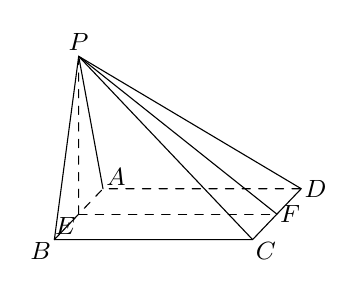
\begin{tikzpicture}[scale=.95,line cap=round,line join=round,font=\small]
  \coordinate (A) at (.65,.68);
  \coordinate (B) at (0,0);
  \coordinate (C) at (2.65,0);
  \coordinate (D) at (3.30,.68);
  \coordinate (E) at (.325,.34);
  \coordinate (F) at (2.975,.34);
  \coordinate (P) at (.325,2.45);

  \draw[dashed] (P) -- (E) -- (A) -- (D);
  \draw[dashed] (E) -- (F);
  \draw (P) -- (A);
  \draw (P) -- (B) -- (E);
  \draw (P) -- (D);
  \draw (P) -- (C);
  \draw (P) -- (F);
  \draw (B) -- (C) -- (F) -- (D);

  \node[above,inner sep=2pt] at (P) {$P$};
  \node[above right,inner sep=1pt] at (A) {$A$};
  \node[below left,inner sep=1pt] at (B) {$B$};
  \node[below right,inner sep=1pt] at (C) {$C$};
  \node[right,inner sep=1pt] at (D) {$D$};
  \node[below left,inner sep=1pt] at (E) {$E$};
  \node[right,inner sep=1pt] at (F) {$F$};
\end{tikzpicture}
\end{center}
\nopagebreak[4]
\Needspace{4\baselineskip}
\textbf{解析}

\gksubpart{（1）}

\Needspace{5\baselineskip}
取底面 A(0,0), B(4,0), C(4,4), D(0,4)，E=(2,0)，P=(2,0,h)。PA=4 且 AB=4，等边三角形条件给
\nopagebreak[4]
\[
h=\sqrt{4^2-2^2}=2\sqrt3.
\]
\Needspace{5\baselineskip}
四棱锥体积为
\nopagebreak[4]
\[
V=\frac13\cdot 4^2\cdot2\sqrt3=\frac{32\sqrt3}{3}.
\]

\gksubpart{（2）}

\Needspace{5\baselineskip}
F=(2,4)，线段 EF 是 PF 在底面上的射影，长度为 4。PF 与底面夹角为 45°，故 PE=4，即 h=4。于是
\nopagebreak[4]
\[
\overrightarrow{PD}=(-2,4,-4),\qquad \overrightarrow{AC}=(4,4,0).
\]
\Needspace{5\baselineskip}
两向量点积为 8，模分别为 6 和 \(4\sqrt2\)，所以
\nopagebreak[4]
\[
\cos\theta=\frac{8}{6\cdot4\sqrt2}=\frac{\sqrt2}{6}.
\]
所求为 \(\arccos(\sqrt2/6)\)。

\gkanswer{答案（1）：$\dfrac{32\sqrt3}{3}$}

\gkanswer{答案（2）：$\arccos\dfrac{\sqrt2}{6}$}

\end{answer}
\begin{answer}
\gksolhead{18}{}

\textbf{题目}：

已知 $A,B,C$ 为 $\triangle ABC$ 的三个内角，$a,b,c$ 是其三条边，$a=2,\cos C=-\frac14$。

（1） 若 $\sin A=2\sin B$，求 $b,c$；

（2） 若 $\cos(A-\frac\pi4)=\frac45$，求 $c$。

\Needspace{4\baselineskip}
\textbf{解析}

\gksubpart{（1）}

\Needspace{5\baselineskip}
正弦定理给 \(a/b=\sin A/\sin B=2\)，因此 b=1。由余弦定理，
\nopagebreak[4]
\[
c^2=a^2+b^2-2ab\cos C=4+1-4(-1/4)=6,
\]
故 c=√6。

\gksubpart{（2）}

\Needspace{5\baselineskip}
\(C=\arccos(-1/4)>90^\circ\)，所以 \(A<\pi-C<\pi/4+\arccos(4/5)\)。由
\nopagebreak[4]
\[
\cos(A-\pi/4)=4/5
\]
\Needspace{5\baselineskip}
有 \(A=\pi/4\pm\arccos(4/5)\)。较大的根不满足三角形内角和限制，故
\nopagebreak[4]
\[
\sin A=\sin(\pi/4-\arccos(4/5))=\frac{\sqrt2}{10}.
\]
\Needspace{5\baselineskip}
同时 \(\sin C=\sqrt{15}/4\)。正弦定理给
\nopagebreak[4]
\[
c=\frac{a\sin C}{\sin A}=\frac{5\sqrt{30}}2.
\]

\gkanswer{答案（1）：$b=1,c=\sqrt6$}

\gkanswer{答案（2）：$c=\dfrac{5\sqrt{30}}2$}

\end{answer}
\begin{answer}
\gksolhead{19}{}

\textbf{题目}：

（1） 团队在 $O$ 点西侧、东侧 20 千米处设有 $A,B$ 两站点，测量距离发现一点 $P$ 满足 $|PA|-|PB|=20$ 千米，可知 $P$ 在 $A,B$ 为焦点的双曲线上，以 $O$ 点为原点，东侧为 $x$ 轴正半轴，北侧为 $y$ 轴正半轴，建立平面直角坐标系，$P$ 在北偏东 $60^\circ$ 处，求双曲线标准方程和 $P$ 点坐标。

（2） 团队又在南侧、北侧 15 千米处设有 $C,D$ 两站点，测量距离发现 $|QA|-|QB|=30$ 千米，$|QC|-|QD|=10$ 千米，求 $|OQ|$（精确到 1 米）和 $Q$ 点位置（精确到 1 米，$1^\circ$）。

\Needspace{4\baselineskip}
\textbf{解析}

\gksubpart{（1）}

\Needspace{5\baselineskip}
设东为 x 正向、北为 y 正向，则 A=(-20,0), B=(20,0)。题设 \(|PA|-|PB|=20>0\)，P 在右支。双曲线焦距 c=20、半焦距 a=10，故 \(b^2=c^2-a^2=300\)，方程为
\nopagebreak[4]
\[
\frac{x^2}{100}-\frac{y^2}{300}=1.
\]
\Needspace{5\baselineskip}
北偏东 60°对应 \(y=x/\sqrt3\)。联立得
\nopagebreak[4]
\[
P=\left(\frac{15\sqrt2}{2},\frac{5\sqrt6}{2}\right)\text{ km}.
\]

\gksubpart{（2）}

\Needspace{5\baselineskip}
对 Q，\(|QA|-|QB|=30>0\) 仍取右支；\(|QC|-|QD|=10>0\) 取上支。两双曲线为
\nopagebreak[4]
\[
\frac{x^2}{225}-\frac{y^2}{175}=1,\qquad
\frac{y^2}{25}-\frac{x^2}{200}=1.
\]
\Needspace{5\baselineskip}
令 \(u=x^2,v=y^2\)，联立得到
\nopagebreak[4]
\[
u=\frac{14400}{47},\qquad v=\frac{2975}{47}.
\]
\Needspace{5\baselineskip}
由于 Q 在第一象限，取 x,y 正根。于是
\nopagebreak[4]
\[
|OQ|=\sqrt{\frac{17375}{47}}\text{ km}
=19.227086\ldots\text{ km},
\]
\Needspace{5\baselineskip}
四舍五入到 1 米为 19,227 米。方位角按正北顺时针计算为
\nopagebreak[4]
\[
\arctan(x/y)=65.55679\ldots^\circ,
\]
取整为北偏东 66°。固定副本参考答案只写约 19 km，精度不满足题面要求。

\gkanswer{答案（1）：$\dfrac{x^2}{100}-\dfrac{y^2}{300}=1$；$P=(\dfrac{15\sqrt2}{2},\dfrac{5\sqrt6}{2})$ 千米。}

\gkanswer{答案（2）：$|OQ|=\sqrt{\dfrac{17375}{47}}$ 千米，按题面取整为 $19227$ 米；$Q$ 位于北偏东 $66^\circ$。}

\end{answer}
\begin{answer}
\gksolhead{20}{}

\textbf{题目}：

已知函数 $f(x)=\sqrt{|x+a|-a}-x$。

（1） 若 $a=1$，求函数的定义域；

（2） 若 $a\ne0$，若 $f(ax)=a$ 有 2 个不同实数根，求 $a$ 的取值范围；

（3） 是否存在实数 $a$，使得函数 $f(x)$ 在定义域内具有单调性？若存在，求出 $a$ 的取值范围。

\Needspace{4\baselineskip}
\textbf{解析}

\gksubpart{（1）}

a=1 时根号内非负要求 \(|x+1|-1\ge0\)，即 \(x\le-2\) 或 \(x\ge0\)。

\gksubpart{（2）}

\Needspace{5\baselineskip}
令 \(y=a(x+1)\)。由 \(f(ax)=a\) 得
\nopagebreak[4]
\[
\sqrt{|y|-a}=y.
\]
必须 y≥0；平方后化为 \(y^2-y+a=0\)。当 a<0 时仅一个根满足 y≥0；当 a>0 时有两个不同的非负根当且仅当 \(0<a<1/4\)。换回 x 与 y 是一一对应的（a$\neq$0），故所求范围为 \(a\in(0,1/4)\)。

\gksubpart{（3）}

\Needspace{5\baselineskip}
若 a<0，记 b=-a>0。定义域为全体实数，并分段为
\nopagebreak[4]
\[
f(x)=
\begin{cases}
\sqrt{2b-x}-x,&x\le b,\\
\sqrt x-x,&x\ge b.
\end{cases}
\]
左支严格递减；右支导数 \(1/(2\sqrt x)-1\)，在 x≥b≥1/4 时非正。故当 b≥1/4，即 a≤-1/4 时，全函数在实数域单调递减。

若 -1/4<a<0，则右支区间从 b<1/4 开始，先递增后递减；a=0 时定义域内 \(\sqrt x-x\) 也非单调；若 a>0，定义域含右支 x≥0，该支同样先递增后递减。因此仅 \(a\in(-\infty,-1/4]\)。

\gkanswer{答案（1）：$(-\infty,-2]\cup[0,+\infty)$}

\gkanswer{答案（2）：$a\in(0,\dfrac14)$}

\gkanswer{答案（3）：$a\in(-\infty,-\dfrac14]$}

\end{answer}
\begin{answer}
\gksolhead{21}{}

\textbf{题目}：

已知数列 $\{a_n\}$ 满足 $a_n\ge0$，对任意 $n\ge2$，$a_n$ 和 $a_{n+1}$ 中存在一项使其为另一项与 $a_{n-1}$ 的等差中项。

（1） 已知 $a_1=5,a_2=3,a_4=2$，求 $a_3$ 的所有可能取值；

（2） 已知 $a_1=a_4=a_7=0$，$a_2,a_5,a_8$ 为正数，求证：$a_2,a_5,a_8$ 成等比数列，并求出公比 $q$；

（3） 已知数列中恰有 3 项为 0，即 $a_r=a_s=a_t=0$，$2<r<s<t$，且 $a_1=1,a_2=2$，求 $a_{r+1}+a_{s+1}+a_{t+1}$ 的最大值。

\Needspace{4\baselineskip}
\textbf{解析}

\Needspace{5\baselineskip}
记 \(d_n=a_n-a_{n-1}\)（n≥2）。题设等价于
\nopagebreak[4]
\[
d_{n+1}=d_n\quad\text{或}\quad d_{n+1}=-\frac12d_n.
\]

\gksubpart{（1）}

在 n=2 处，\(a_3\) 可为 \(2a_2-a_1=1\) 或 \((a_1+a_2)/2=4\)。在 n=3 处，结合 a₂=3、a₄=2，\(a_3\) 可为 \((a_2+a_4)/2=5/2\) 或 \(2a_4-a_2=1\)。两组候选取交集得唯一值 a₃=1。

\gksubpart{（2）}

\Needspace{5\baselineskip}
在零项 a₄ 周围，非负性与 a₂>0 排除 \(a_4=(a_3+a_5)/2\)，故 \(a_3=(a_2+a_4)/2=a_2/2\)。同理围绕 a₄ 得 \(a_5=a_3/2=a_2/4\)。再围绕 a₇，得到 \(a_6=a_5/2\)、\(a_8=a_6/2=a_2/16\)。所以
\nopagebreak[4]
\[
\frac{a_5}{a_2}=\frac{a_8}{a_5}=\frac14,
\]
三数成等比数列，公比为 1/4。

\gksubpart{（3）}

\Needspace{5\baselineskip}
记 \(d_n=a_n-a_{n-1}\)。在任意零项 \(a_r=0\) 处，相邻项非负及差分规则强制 \(d_r<0\)、\(d_{r+1}=-d_r/2>0\)，所以
\nopagebreak[4]
\[
a_{r+1}=-\frac{d_r}{2}=\frac{a_{r-1}}2.
\]
\Needspace{5\baselineskip}
从 \(a_1=1,a_2=2\) 出发，所有差分绝对值不增。第一次出现负差时，它由正差取相反数的一半得到，故其绝对值至多 \(1/2\)；第一个零后的项因此至多为 \(1/4\)。设某零项之后的正差为 \(p=a_{r+1}>0\)，在到达下一个零项 \(a_s=0\) 前，差分可以保持 \(p\)、减小或变号；一旦变为负差，其绝对值至多为 \(p/2\)，之后无论变号与否绝对值都不增。因此 \(0<a_{s+1}=-d_s/2\le p/4\)。三个零后的正项依次至多为 \(1/4,1/16,1/64\)，故三项和不超过
\nopagebreak[4]
\[
\frac14+\frac1{16}+\frac1{64}=\frac{21}{64}.
\]
等号可达：令 d₂=1，d₃=d₄=d₅=d₆=-1/2，d₇=1/4，d₈=d₉=-1/8，d₁₀=1/16，d₁₁=d₁₂=-1/32，d₁₃=1/64，此后令差值恒为 1/64。所得序列非负且恰在第 6、9、12 项为零，三个零后的项分别为 1/4、1/16、1/64，达到上界 21/64。

\gkanswer{答案（1）：$a_3=1$}

\gkanswer{答案（2）：$q=\dfrac14$}

\gkanswer{答案（3）：$\dfrac{21}{64}$}

\end{answer}